\documentclass[10pt,twoside,openany,final]{memoir}
\usepackage[utf8]{inputenc}
\usepackage[pass]{geometry}
\usepackage[T1]{fontenc}
\usepackage[english]{babel}
\usepackage{amsmath}
\usepackage{amsfonts}
\usepackage{amsthm}
\usepackage{subcaption}
\usepackage[labelformat=parens,labelsep=quad,skip=3pt]{caption}
\usepackage{amssymb} 
\usepackage[usenames,dvipsnames]{xcolor}
\usepackage{graphicx}
\usepackage{hyperref}
\usepackage[all]{xy}
\usepackage{tikz-cd}
\usepackage[citestyle=authoryear,backend=bibtex]{biblatex}
\usepackage{filecontents}
\usepackage[english, status=draft]{fixme}
\fxusetheme{color}
\usepackage{cleveref} 
\usepackage{tensor}
\usepackage[backgroundcolor=cyan]{todonotes}
\usepackage{wallpaper}
\usepackage{titlesec}
%\usepackage[bottom=1in,left=1.22in,right=1.63in,showframe]{geometry}
\bibliography{bib}
\titleformat{\chapter}[display]
{\center\normalfont\bfseries}{}{0pt}{\Large}

\renewcommand\chaptermarksn[1]{}
\newcommand{\ssection}[1]{%
\newpage%
\section[#1]{\centering\normalfont\scshape \textbf{#1}}}

\newcommand{\sssection}[1]{%
\section[#1]{\centering\normalfont\scshape \textbf{#1}}}
\addtolength{\textwidth}{30pt}
\addtolength{\foremargin}{-30pt}
\checkandfixthelayout

\setlength{\parindent}{0em}
\setlength{\parskip}{1em}
\renewcommand{\baselinestretch}{1}

\usepackage{scalerel,stackengine}
\stackMath
\newcommand\reallywidehat[1]{%
\savestack{\tmpbox}{\stretchto{%
  \scaleto{%
    \scalerel*[\widthof{\ensuremath{#1}}]{\kern-.6pt\bigwedge\kern-.6pt}%
    {\rule[-\textheight/2]{1ex}{\textheight}}%WIDTH-LIMITED BIG WEDGE
  }{\textheight}% 
}{0.5ex}}%
\stackon[1pt]{#1}{\tmpbox}%
}
\parskip 1ex

\newtheoremstyle{break}
{\topsep}{\topsep}
{\itshape}{}
{\bfseries}{}
{\newline}{}
\theoremstyle{definition}
\newtheorem{theorem}{Theorem}[chapter]
\newtheorem{lemma}[theorem]{Lemma}
\newtheorem{proposition}[theorem]{Proposition}
\newtheorem{corollary}[theorem]{Corollary}
\newtheorem{definition}[theorem]{Definition}
\newtheoremstyle{Break}
{\topsep}{\topsep}
{}{}
{\bfseries}{}
{\newline}{}
\theoremstyle{Break}
\newtheorem{example}[theorem]{Example}
\newtheorem*{remark}{Remark}
\newtheorem*{note}{Note}
\setcounter{secnumdepth}{0}
\usepackage{xpatch}
\xpatchcmd{\proof}{\ignorespaces}{\mbox{}\\\ignorespaces}{}{}
%\newenvironment{Proof}{\proof \mbox{} \\ \\ *}{\endproof}

\chapterstyle{thatcher}

\newenvironment{abst}{\rightskip1in\itshape}{}

\makepagestyle{abs}
\makeevenhead{abs}{}{}{}
\makeoddhead{abs}{}{}{}
\makeevenfoot{abs}{}{\scshape I }{}
\makeoddfoot{abs}{}{\scshape  I }{}
%\makeheadrule{abs}{\textwidth}{\normalrulethickness}
%\makefootrule{abs}{\textwidth}{\normalrulethickness}{\footruleskip}
\pagestyle{abs}


\makepagestyle{cont}
\makeevenhead{cont}{}{}{}
\makeoddhead{cont}{}{}{}
\makeevenfoot{cont}{}{\scshape II }{}
\makeoddfoot{cont}{}{\scshape  II }{}
%\makeheadrule{abs}{\textwidth}{\normalrulethickness}
%\makefootrule{abs}{\textwidth}{\normalrulethickness}{\footruleskip}
\pagestyle{cont}

\newcommand{\lv}{\left\lVert}
\newcommand{\rv}{\right\rVert}


\renewcommand\chaptermarksn[1]{}
\nouppercaseheads
\createmark{section}{left}{shownumber}{}{.\space}
\makepagestyle{dut}
\makeevenhead{dut}{Malthe Karbo\scshape\rightmark}{}{\scshape\leftmark}
\makeoddhead{dut}{\scshape\leftmark}{}{Malthe Karbo\scshape\rightmark}
\makeevenfoot{dut}{}{\scshape $-$ \thepage\ $-$}{}
\makeoddfoot{dut}{}{\scshape $-$ \thepage\ $-$}{}
\makeheadrule{dut}{\textwidth}{\normalrulethickness}
\makefootrule{dut}{\textwidth}{\normalrulethickness}{\footruleskip}
\pagestyle{dut}

\makepagestyle{chap}
\makeevenhead{chap}{}{}{}
\makeoddhead{chap}{}{}{}
\makeevenfoot{chap}{}{\scshape $-$ \thepage\ $-$}{}
\makeoddfoot{chap}{}{\scshape $-$ \thepage\ $-$}{}
\makefootrule{chap}{\textwidth}{\normalrulethickness}{\footruleskip}
\copypagestyle{plain}{chap}

\newcommand{\R}{\mathbb{R}}
\newcommand{\C}{\mathbb{C}}
\newcommand{\N}{\mathbb{N}}
\newcommand{\mbr}{(X,\mathcal{A})}
\newcommand{\Z}{\mathbb{Z}}
\newcommand{\Q}{\mathbb{Q}}
\newcommand{\F}{\mathcal{F}}
\newcommand{\G}{\widehat{G}}
\newcommand{\A}{\mathcal{A}}
\newcommand{\B}{\mathbb{B}}
\newcommand{\dd}{\partial}
\newcommand{\ee}{\epsilon}
\newcommand{\la}{\lambda}
\newcommand{\U}{\mathcal{U}}
\newcommand{\cc}{\text{C}_{\text{c}}}
\renewcommand{\H}{\mathcal{H}}
\renewcommand{\P}{\mathcal{P}}
\renewcommand{\S}{\mathcal{S}}
\newcommand{\Prob}{\mathrm{Prob}}
\DeclareMathOperator{\Aut}{Aut}
\DeclareMathOperator{\Ext}{Ext}
\DeclareMathOperator{\supp}{supp}
\newcommand{\PM}{\mathrm{PM}}
\renewcommand{\d}{\mathrm{d}}
\renewcommand{\Re}{\mathrm{Re}}
\renewcommand{\Im}{\mathrm{Im}}
\DeclareMathOperator{\tr}{Tr}
\DeclareMathOperator{\Tr}{Tr}
\DeclareMathOperator{\Span}{span}
\makeatletter
\newcommand{\Spvek}[2][r]{%
\gdef\@VORNE{1}
\left(\hskip-\arraycolsep%
\begin{array}{#1}\vekSp@lten{#2}\end{array}%
\hskip-\arraycolsep\right)}

\def\vekSp@lten#1{\xvekSp@lten#1;vekL@stLine;}
\def\vekL@stLine{vekL@stLine}
\def\xvekSp@lten#1;{\def\temp{#1}%
\ifx\temp\vekL@stLine
\else
\ifnum\@VORNE=1\gdef\@VORNE{0}
\else\@arraycr\fi%
#1%
\expandafter\xvekSp@lten
\fi}
\makeatother

\newcommand{\K}{\mathbb{K}}
\addtocontents{toc}{\protect\thispagestyle{empty}} 
\def\acts{\curvearrowright}


\pagenumbering{arabic}
\begin{document}
%\tableofcontents
\clearpage
\thispagestyle{empty}

\begin{titlingpage}
	\ThisLRCornerWallPaper{1}{frontpage/1.pdf}	
	\vspace*{5.5cm}
	\noindent
	{\large\textsc{Malthe Munk Karbo}}\\[0.5cm]
	{\large\textsc{Simplicity of Crossed Products of $C^*$-algebras}}\\[0.1cm]
	\vfill\noindent
	{\large\textsc{Masters thesis in mathematics}}\\[0.2cm]
	\noindent
	{\large\textsc{Department of Mathematical Sciences}}\\[0.2cm]
	\noindent
	{\large\textsc{University of Copenhagen}}\\[1cm]
	{\large\textsc{Advisor \\[0.2cm] {\Large Søren Eilers }}}\\[1cm]
	{\large\textsc{December 7, 2018}}
	\let\cleardoublepage\clearpage
\end{titlingpage}
\normalfont
\restoregeometry
\cleardoublepage

%\include{abstract{abs}}
\newpage

\begin{KeepFromToc}
\chapter*{Introduction}
In fields like statistics, machine learning and alike, we are often interested in measuring how 'equal' certain objects are - e.g., observed data, and occasionally this is the goal of a statistician is to find a function which allows him to measure this. There is a rich theory of normed spaces and Hilbert spaces, which aids in this process. We will in this paper introduce and discuss the theory of \emph{Reproducing Kernel Hilbert Spaces}, which is a class of Hilbert spaces stemming from a certain class of functions, called \emph{kernels}, which in a suitable fashion generalizes the notion of an inner product. We then move on to show a result called the 'Representer Theorem', which characterizes the solutions to certain problems in a nice way, and some generalizations of it.
	  \tableofcontents
\end{KeepFromToc}


\chapter{Kernel theory}
In this paper, we will restrict ourselves to working with real Hilbert spaces and real-valued functions, however, it is entirely possible to develop theory discussed in the following for complex Hilbert spaces. 

\sssection{Reproducing Kernels}
We will denote Hilbert spaces by $\H$, and by $\mathcal{X}$ we will denote any non-empty set - usually refered to as a sample space. The goal of this section is to characterize a certain kind of Hilbert space of functions through a class of functions called \emph{kernels}:
\begin{definition}
	A Hilbert space $\H$ of functions $f \colon \mathcal{X} \to \R$ is called a \emph{reproducing kernel Hilbert space} (RHKS) if the evaluation functional $f \mapsto f(x)$ is continuous.
\end{definition}
The term \textit{kernel} comes from a connection with a class of certain compact operators on a Hilbert space, called integral operators - which is usually defined pointwise by integration against a function initially refered to as an integral kernel. 

By the Riesz Representation theorem, there is a unique vector $ev_x \in \H$ such that the evaluation $f \mapsto f(x)$ is given by $\langle f , ev_x\rangle$ for $f \in \H$, whenever $\H$ is a RKHS. An important distinguishment between general Hilbert spaces and RKHS's is the following:
\begin{lemma}
	Let $\H$ be a RKHS in over $\mathcal{X}$, and let $ (f_n) \subseteq \H$. If $f_n \to f$ in norm, then $f_n(x) \to f(x)$ for all $x \in \H$.
	\label{paul3.2}
\end{lemma}
\begin{proof}
	For all $x \in \mathcal{X}$ and $f_n, f$ as above, we get by Cauchy-Schwarz that
	\begin{align*}
		|f_n(x) - f(x) | = | \langle f_n-f , ev_x \rangle| \leq \lv f_n - f \rv \lv ev_x \rv \to 0.
	\end{align*}
\end{proof}
We are interested in a special kind of kernel functions, namely so called positive-definite ones:
\begin{definition}
	A symmetric function $k \colon \mathcal{X} \times \mathcal{X} \to \R$ such that given any non-empty finite subset $F \subseteq \mathcal{X}$, the matrix $(k(x,y))_{x,y \in F}$ is positive semi-definite is called a \emph{positive-definite kernel} on $\mathcal{X}$.
\end{definition}
Given a symmetric function $k$ on $\mathcal{X}$, then for fixed $y \in \mathcal{X}$ we will use $k_y$ to denote the function $k(\cdot,y)$, whenever this imposes no confusion. This will be convenient later on.

There is a correspondance between positive-definite kernels on $\mathcal{X}$ and reproducing spaces over $\mathcal{X}$, as we will see:
\begin{proposition}
	Given a positive-definite kernel $k$ on $\mathcal{X}$, there is a reproducing kernel Hilbert space $\H_k\subseteq \R^{\mathcal{X}}$ such that the evaluation functional is given by $f(x) = \langle f, k_x\rangle$ for $f \in \H_k$ and $x \in \mathcal{X}$.
	\label{moore}
\end{proposition}
\begin{proof}
	If we set $\H_0 := \Span_\R\left\{ k_x \ \big| x \in \mathcal{X} \right\}$, then we obtain a pre-Hilbert space with respect to the Hermitian form defined by
	\begin{align*}
		\left\langle \sum_i \alpha_i k(\cdot , y_i) , \sum_j \beta_j k(\cdot, x_j) \right\rangle := \sum_{i,j}\alpha_i \beta_j  k(y_i,x_j),
	\end{align*}
	since $k$ is positive definite and symmetric: It is easy to see that if $f \in \H_0$ - i.e., $f \colon x \mapsto \sum_{i=1}^n \alpha_i k_{x_i}(x)$ for some $x_i \in \mathcal{X}$ and $\alpha_i \in \R$, then for $x \in \mathcal{X}$ we have
	\begin{align*}
		\langle k(\cdot , x ) , f \rangle = f(x),
	\end{align*}
	and since $k$ is positive definite, we have $k(x,y)^2 \leq k(x,x)k(y,y)$. Hence, for $x \in \mathcal{X}$ we see that $|f(x)|^2=|\langle k(\cdot , x ) , f \rangle|^2 \leq | k(x,x) \langle f,f \rangle|$ so that $\langle f,f \rangle = 0 \iff f=0$.

	Let $\H_k$ denote the Cauchy completion of $\H_0$ with respect to $\langle \cdot , \cdot \rangle$, and denote also the inner product extension to $\H_k$ by $\langle \cdot , \cdot \rangle$. We wish to show that $\H_k$ is in fact a RKHS. So let $h \in \H_k$ and pick any Cauchy sequence $(f_n) \subseteq \H_0$ such that $f_n \to f$. For $x \in \mathcal{X}$, let $h(x) := \lim_n f_n(x)$. By Cauchy-Schwarz:
	\begin{align*}
		|\langle f_n - f_m , k_x\rangle| \leq \lv f_n - f_m \rv \lv k(x,x)\rv \to 0, \text{ for } x \in \mathcal{X},\text{ as }n,m \to \infty,
	\end{align*}
	so $h(x) \in \R$ is well-defined, and it is clear that $x \mapsto h(x)$ is independent on the choice of Cauchy representant $(f_n)$ of $h$. Hence we may view $\H_k$ as a subset of $\R^{\mathcal{X}}$.
	Furthermore, if $h$ and $(f_n)$ is as above, then 
	\begin{align*}
		\langle h , k_x \rangle = \lim_n \langle f_n , k_x \rangle = \lim_{n\to \infty} f_n(x) =h(x), \text{ for } x \in \mathcal{X}, 
	\end{align*}
	and since $k_x \in \H_k$, Riesz Representation theorem says that $\H_k$ is a RKHS.
\end{proof}
If $\H$ is a RKHS over $\mathcal{X}$, then the evaluation functional $\delta_x$ is, by the Riesz Representation theorem, given by some element $k_x \in \H$. Then the map $k \colon \mathcal{X} \times \mathcal{X} \to \R$, $k(x,y):= k_y\left( x \right)$, is clearly symmetric and if $\alpha \in \R^n$ and $x_1,\dots,x_n \in \mathcal{X}$, then 
\begin{align*}
	\sum_{i,j}\alpha_i \alpha_j k(x_i,x_j) = \lv \sum_i \alpha_i k_{x_i} \rv^2 \geq 0,
\end{align*}
so it is a positive definite kernel. The correspondance between positive definite kernels and RKHS is in fact one-to-one. This follows from the following:
\begin{lemma}
	If $\H_k$ is a RKHS over $\mathcal{X}$, then $\Span_\R\left\{ k_x \ | \ x \in \mathcal{X} \right\}$ is dense in $\H_k$.
	\label{paul3.1}
\end{lemma}
\begin{proof}
	The orthogonal complement of the span is equal to zero, since $\H_k$ is reproducing since $f \perp k_x \implies f(x)=0$ for $x \in \mathcal{X}$ and $f \in \H_k$. Hence the span is dense in $\H_k$. 
\end{proof}
\begin{proposition}
	If $\H_1, \H_2$ are RKHS's over $\mathcal{X}$ such that their kernels $k_1$ and $k_2$ are equal, then $\H_1 = \H_2$ and $\lv f \rv_{\H_1} = \lv f \rv_{\H_2}$.
\end{proposition}
\begin{proof}
	By \Cref{paul3.1}, we see that $V_i = \Span_\R \left\{ k_{x} \in \H_i \ | \ x \in \mathcal{X} \right\}$ is dense in $H_i$, $i = 1,2$, and $f \in V_i$ is independent of the choice of $i$, since $f(x) = \sum_{k} \alpha_k k_{x_k}(x)$ for some $\alpha_j \in \R$ and $x_j \in \mathcal{X}$, so $V_1=V_2$ in $\R^{\mathcal{X}}$, and if $f = \sum_j \alpha_j k_{x_j} \in V_1$ then 
	\begin{align*}
		\lv f \rv_{\H_1} = \sum_{i,j} \alpha_j \alpha_i k(x_i,x_j) = \lv f \rv_{\H_2}.
	\end{align*}
	Let $f \in \H_1$, and pick a sequence $f_n \subseteq V_1$ such that $f_n \to f$ in $\H_1$. By the above, $f_n$ is Cauchy in $V_2$ and hence $\H_2$, with limit $g \in \H_2$. Then, by \Cref{paul3.2} we have
	\begin{align*}
		f(x) = \lim_n f_n(x) = g(x), \ x \in \mathcal{X}.
	\end{align*}
	By symmetry, we see that $\H_1 = \H_2$, and since the norms agree on a dense set, they agree on the equal closures.
\end{proof}
Hence, we may characterize RKHS's over $\mathcal{X}$ as a pair $(\H_k,k)$ or simply $\H_k$, for some positive-definite kernel $k$ on $\mathcal{X}$, where the space $\H_k$ is the space defined in \Cref{moore}. This space is called the \emph{canonical kernel space}. 

It is easy to represent the kernel $k$ of a RKHS $\H_k$ in terms of a ONB:
\begin{theorem}
	Let $\H_k$ be a RKHS, and let $(e_i)_{i \in I}$ be an ONB for $\H_k$. Then $k(x,y) = \sum_{i \in I} e_i(y) e_i(x)$, for $x, y \in \mathcal{X}$.
	\label{paul3.4}
\end{theorem}
\begin{proof}
	It holds that $e_i(x) = \langle k_x , e_i\rangle$, hence expanding into Fourier coefficients we see that $k_y = \sum_{i \in I}e_i(y) e_i$. The theorem follows since norm convergence implies point-wise convergence in a RKHS.
\end{proof}

We may also construct RKHS in a different way: Given a set $\mathcal{X}$, a Hilbert space $\H$ and a map $\varphi \colon \mathcal{X} \to \H$, if we define $k \colon \mathcal{X} \times \mathcal{X} \to \R$ by 
\begin{align*}
	k(x,y) := \langle \varphi(x), \varphi(y) \rangle, \text{ for } x,y \in \mathcal{X},
\end{align*}
then $k$ is a positive-definite kernel giving rise to a RKHS. While $k$ is uniquely determined by its canonical RKHS $\H_k$, there may be other maps $\psi \colon \mathcal{X} \to \H'$ inducing the same kernel. In this setup, the map $\varphi$ is called a \emph{feature map} and $\H$ is called a \emph{feature space}. Clearly, given a RKHS $\H_k$, the map $x \mapsto k_x$, is a feature map with feature space $\H_k$. We also say that $\H_k$ is the canonical feature space of $k$ and $\mathcal{X}$.

\sssection{Examples and constructions of RKHS and kernels}
We will now cover a few important examples of both kernels and RKHS's and ways to define new kernels and RKHS's from old ones.
\begin{lemma}
	If $k_1$ and $k_2$ are kernels on $\mathcal{X}$, then $k=k_1+k_2$ is a kernel and it's RKHS is the algebraic product $\H = \H_{k_1} + \H_{k_2}$ with norm 
	\begin{align}
		\lv f \rv_\H^2 = \min_{(f_1,f_2) \in \H_{k_1}\oplus \H_{k_2}} \left\{ \lv f_1\rv_{\H_{k_1}}^2 + \lv f_2 \rv_{\H_{k_2}}^2  \right\} \label{eqkernsum}
	\end{align}
	\label{sumkern}
\end{lemma}
\begin{proof}
	Let $\H'=\H_{k_1} \oplus \H_{k_2}$ equipped with the natural inner product and $\pi$ be the canonical surjection onto $\H$, i.e., $s \colon (f,g) \mapsto f+g$. Then the nullspace of $\mathcal{N}(\pi)=\{f \oplus -f \mid f \in H_{k_1} \cap H_{k_2} \}$ of $\pi$ is closed, for if $(f_n,-f_n)_n \subseteq \mathcal{N}(s)$ converges in $\H'$ to a pair $(f,g)$, then $f_n \to f$ and $-f_n \to g$ in $\H_{k_1}$ and $\H_{k_2}$, respectively, and therefore also pointwise everywhere, so $f(x)=-g(x)$ for all $x \in \mathcal{X}$. We may then write $\H' = \mathcal{N}(s) \oplus \mathcal{N}(s)^\perp$, and we may identify $\H$ with $\mathcal{N}(s)^\perp$ as Hilbert spaces.

	Now, let $P$ denote the orthogonal projection onto $\mathcal{N}(s)^\perp$. Then, by definition of the orthogonal projection, we see that \Cref{eqkernsum} holds, and for $f,g \in \H$, we have $\langle f,g \rangle_{\H} = \langle P(f_0,f_1), P(g_0,g_1)\rangle_{\H'}$, where $f=P(f_0,f_1)$ and $g=P(g_0,g_1)$.

	It remains to be shown that $\H$ is a RKHS with kernel $k$. Note that for all $x$ we have $(k_{1}(\cdot, x ) , k_2(\cdot,x)) \perp \mathcal{N}(s)$, since the inner product with $(f,-f)$ equals $f(x)-f(x)=0$. If $f = f_1+f_2 \H$ then 
	\begin{align*}
		\langle f, k_x \rangle_{\H} = \langle P(f_1,f_2) , P(k_{1}(\cdot, x ) , k_2(\cdot , x)) \rangle_{\H'} &= \langle (f_1,f_2) , (k_1(\cdot,x),k_2(\cdot,x))\rangle_{\H'}\\
		&= \langle f_1 , k_{1}(\cdot,x)\rangle_{\H_1}+ \langle f_2, k_{2}(\cdot,x) \rangle_{\H_2} \\
		&= f_1(x)+f_2(x)=f(x),
	\end{align*}
	finishing the proof.
\end{proof}
\begin{lemma}
	If $k_1$ and $k_2$ are kernels on $\mathcal{X}$, then $k=k_1 \otimes k_2$, given by $\mathcal{X}\times \mathcal{X} \ni \left( x,y \right) \mapsto k_1(x,y)k_2(x,y)$, is a kernel.
	\label{productkern}
\end{lemma}
\begin{proof}
	First note that if $\H_1$ and $\H_2$ are the RKHS of $k_1$ and $k_2$ respectively, then their Hilbert space tensor product $\H= \H_1 \otimes \H_2$ with inner product defined on simple tensors $g\otimes h , g' \otimes h'$ by $\langle g \otimes h , g' \otimes h'\rangle_\H := \langle g , g \rangle_{\H_1} \langle h, h' \rangle_{\H_2}$ is again a RKHS, since for $g\otimes h \in \H$ and $(x,y) \in \mathcal{X} \times \mathcal{X}$, we have
	\begin{align*}
		g \otimes h (x,y) = g(x) h(y) = \langle g , k_1(\cdot,x)\rangle_{\H_1} \langle h , k_2(\cdot,y)\rangle_{\H_2} = \langle g \otimes h , k_1(\cdot,x)k_2(\cdot,y)\rangle_{\H},
	\end{align*}
	and since the inner product is defined pointwise and the simple tensors span a dense subset of $\H$, we obtain the desired. Moreover, $k$ is clearly symmetric and also positive definite, for if $\varphi(x) := k_1(\cdot,x) \otimes k_2(\cdot,x)$, then 
	\begin{align*}
		k(x,y) = k_1(x,y) k_2(x,y) &= \langle k_{1}(\cdot,x), k_{1}(\cdot,y)\rangle_{\H_1} \langle k_{2}(\cdot,x),k_{2}(\cdot,y)\rangle_{\H_2} \\ 
		&= \langle k_{1}(\cdot,x) \otimes k_{2}(\cdot,x)\rangle, k_{1}(\cdot,y) \otimes k_{2}(\cdot,y)\rangle_{\H}\\
		&= \langle \varphi(x), \varphi(y)\rangle_{\H}.
	\end{align*}
	Alternatively, it follows since $a^*a \otimes b^*b = (a^* \otimes b^*)(a \otimes b) \geq 0$ whenever $a,b$ are bounded linear operators on Hilbert spaces $\H, \mathcal{K}$ respectively, so given any finite set $F \subseteq \mathcal{X}$, the matrix $(k(x,y))_{x,y \in F}=(k_1(x,y))_{x,y \in F} \otimes (k_2(x,y))_{x,y \in F}$, which consequently must be of the form $a^*a \otimes b^*b$ for suitable matrices.
\end{proof}

We end with some examples of canonical kernels:
\begin{example}\mbox{\\}
	\begin{enumerate}
		\item If $\lambda>0$ and $k$ is a kernel on $\mathcal{X}$, then $\lambda k$ is a kernel on $\mathcal{X}$.
		\item If $(k_n)_{n \in \N}$ is a sequence of kernels on $\mathcal{X}$ such that the limit $k(x,y):=\lim_{n} k_n(x,y)$ exists for all $x,y \in \mathcal{X}$, then $k$ is a kernel on $k$.
		\item If $f \colon \mathcal{X} \to \R$ is any function and $k$ is a kernel on $\mathcal{X}$, then the function $\tilde{k}(x,y) := f(x) k(x,y) f(y)$ is a kernel on $\mathcal{X}$.
		\item If $\mathcal{X} = \R^n$, then $(x,y) \mapsto \langle x,y \rangle ^k$ is a kernel on $\mathcal{X}$ called the \emph{polynomial kernel of degree $k$ on $\mathcal{X}$}.
		\item If $k$ is a kernel on $\mathcal{X}$, then $k'(x,y) := e^{k(x,y)}$ is a kernel on $\mathcal{X}$ called the \emph{exponential kernel} of $k$.
		\item For $\lambda > 0$ and $\mathcal{X} = \R^n$, then the function $k(x,y) = e^{-\lambda \lv x-y \rv^2}$ is a kernel called the \emph{radial basis function kernel (RBF kernel)} with bandwidth $\lambda > 0$ (often parametrized with $\lambda = \frac{1}{2 \sigma^2}$).
	\end{enumerate}
\end{example}
\begin{proof}
	\textbf{1:} If $\varphi$ is a feature map for $k$, let $\Phi = \sqrt{\lambda} \varphi$, then $\Phi$ is a featuremap for $\lambda k$.

	\textbf{2:} Clearly the limit will be symmetric and positive semi-definite.

	\textbf{3:} Let $\varphi$ be a feature map associated to $k$, and let $\Phi \colon x \mapsto f(x)\varphi(x)$ for $x \in \mathcal{X}$, then $\tilde{k}(x,y) = \langle \Phi(x), \Phi(y)\rangle$ is the desired kernel

	\textbf{4:} This follows from repeated use of \Cref{productkern} applied to $k(x,y) = \langle x, y \rangle$.

	\textbf{5:} For $N \geq 0$, we see that $\sum_{m=0}^N \frac{1}{m!}k(x,y)^m$ defines a kernel by (1), \Cref{sumkern} and \Cref{productkern}. By (2), we see that 
	\begin{align*}	
		e^{k(x,y)}=\sum_{m=0}^\infty \frac{1}{m!}k(x,y)^m = \lim_{N \to \infty} \sum_{m=0}^N \frac{1}{m!}k(x,y)^m,
	\end{align*}
	is a kernel.

	\textbf{6:} This follows from the identity
	\begin{align*}
		k(x,y) = e^{-\lambda \lv x-y \rv^2} = e^{-\lambda \lv x \rv^2} e^{2 \lambda \langle x,y \rangle} e^{- \lambda \lv y \rv^2}
	\end{align*}
	which is a kernel by (3) and (5) and (1).
\end{proof}

In the following, we let 
\begin{align*}
	\H = \left\{ f \in \mathrm{AC}([0,1],\R) \mid f' \in L^2([0,1]), \ f(0) = 0  \right\},
\end{align*}
where $\mathrm{AC}([0,1],\R)$ is the space of absolutely continuous functions $f \colon [0,1] \to \R$. Note that we only require $f'$ to be a function satisfying $f(x) = \int_0^x f'(t)\d t$ (i.e., an almost everywhere derivative of $f$).
\begin{example}
	The space $\H$ is a RKHS when given inner product $\langle f,g\rangle_\H := \langle f' , g' \rangle_{L^2([0,1])}$, and its reproducing kernel is the kernel $k \colon [0,1] \times [0,1] \to [0,1]$ , $k(x,y) = \min(x,y)$.
\end{example}
\begin{proof}
	For $f \in \H$, it holds that $f(x)=f(0)+\int_0^x f'(t) \d t = \int_0^x f'(t) \d t$ for $x \in [0,1]$, so
	\begin{align}
		|f(x)| = \left| \int_0^x f'(t) \d t \right| = |\langle 1_{[0,x]},f' \rangle_{L^2}| \leq x^{\frac12} \lv f \rv_{\H} \label{Cauchy}
	\end{align}
	Thus $f = 0 $ in $\H$ implies $f = 0$. The remaining properties making $\langle \cdot , \cdot \rangle_{\H}$ an inner product are immediate from the definition, and $\H$ is clearly a space of functions. It remains to be shown that $\H$ is complete in the norm induced by the inner product: Let $(f_n)$ be a Cauchy-sequence in $\H$ so that $(f_n')$ is Cauchy in $L^2([0,1])$ with limit $g \in L^2([0,1])$. By \Cref{Cauchy} it holds that $f_n(x)$ is Cauchy in $\R$ for all $x \in [0,1]$, hence we may define $f \colon [0,1] \to \R$, $x \mapsto \lim_n f_n(x)$. To see that $f$ is absolutely continuous, note first that $f(0) = \lim_n f_n(0)=0$, and we calculate for $x \in [0,1]$:
	\begin{align*}
		f(x) = \lim_n \int_0^x f_n'(t) \d t = \int_0^x g(t) \d t,
	\end{align*}
	so $f(x) = f(0) + \int_0^x g(t) \d t$, and $g$ is measurable, hence $f$ is absolutely continuous on $[0,1]$ and has a derivative $f'$ almost everywhere satisfying $f' = g$ almost everywhere, so $f' \in L^2([0,1])$. Hence $f \in \H$ and
	\begin{align*}
		\lv f - f_n \rv_{\H} =  \lim_n \lv f_n' - g \rv_{L^2} = 0,
	\end{align*}
	so $\H$ is complete, i.e., a Hilbert space. We proceed to show that $k$ is a reproducing kernel for $\H$: Fix $x \in [0,1]$, the function $k_x$ satisfies $k_x(0)=0$ and is clearly absolutely continuous on $[0,1]$ with a single discontinuity point at $x$ and the almost everywhere defined partial derivative $k_x' = 1_{[0,x]}$ clearly satisfying $k_x' \in L^2([0,1])$, so $k_x \in \H$. For any $f \in \H$, we see that
	\begin{align*}
		f(x) = \int_0^x f'(t) \d t = \int_0^1 f'(t) k_x'(t) \d t = \langle f,k_x \rangle_{\H},
	\end{align*}
	so $\H$ is a reproducing kernel space with kernel $k$.
\end{proof}
The above example generalizes to a more general form: For $m\geq 1$ let
\begin{align*}
	W_0^m:= \left\{ f \colon [0,1] \to \R \mid f^{(n)} \in \mathrm{AC}([0,1],\R), \ f^{(n)}(0)=0 \text{ for } \ 0 \leq n \leq m-1 \text{ and } f^{(m)} \in L^2([0,1] \right\}.
\end{align*}
Then $W_0^m$ is a RKHS with norm $\lv f \rv_{W_0^m} = \lv f^{(m)} \rv_{L^2}$. The reproducing kernel of $W_0^m$ can be found by examining the problem:
\begin{align*}
	f^{(m)}=g, \ f \in W_0^m.
\end{align*}
We denote the associated Green's function by $G_m$, i.e., a function $[0,1]^2 \to \R$ such that $f(x) = \int_{0}^1 G_m(x,t)g(t) \d t$.  It can be shown that 
\begin{align*}
	G_m(x,y) = 1_{[0,x]}(y)(x-y)^{m-1}((m-1)!)^{-1},
\end{align*}
 and that the function $k_m(x,y) = \int_{0}^1 G_m(x,t) G_m(y,t) \d t$ is the reproducing kernel for $W_0^m$. In the case for $m=1$, we recover the above example.

Let $M(\R^n)$ denote the set of all finite complex-valued Borel measures. For $\mu \in M(\R^n)$, the Fourier transformation of $\mu$ is the function $\widehat{\mu} \in C_b(\R^n)$ given by
\begin{align*}
	\widehat{\mu}(w)=\int_{\R^n} e^{-i\langle w, t\rangle_{\R^n}} \d \mu(t), \ \text{for } w \in \R^n.
\end{align*}
This allows us to obtain the following theorem, due to Bochner:
\begin{theorem}[Bochner's Theorem]
	For a continuous function $\varphi \colon \R^n \to \R$, the kernel $k(s,t) := \varphi(s-t)$ is positive definite if and only if there is a positive finite Borel measure $\mu$ on $\R^n$ such that $\varphi = \widehat{\mu}$.
	\label{bochner}
\end{theorem}
For proof, see \cite{ACIAHA}. Bochners thereom allows us to completely characterize the RKHS's of kernels given by $k(s,t)=\varphi(s-t)$ for certain continuous functions $\varphi \colon \R^n \to \R$, for instance the RKHS to the RBF kernel.
\begin{theorem}
	Let $\varphi \colon \R^n \to \R$ be a continuous function with $\varphi \in L^1(\R^n)$ and its Fourier transform $\widehat{\varphi} \in L^1(\R^n)$ such that the function $k(s,t):= \varphi(s-t)$ is a positive definite kernel. For $f \in L^2(\R^n)\cap L^1(\R^n)$ define the number
\begin{align*}
	\lv f \rv_k^2:= (2\pi)^{-n} \int_{\R^n}\frac{|\hat{f}(w)|^2}{\hat{\varphi}(w)} \d w,
\end{align*}
	Then the RKHS associated to $k(s,t) = \varphi(s-t)$ is the set of functions
	\begin{align*}
		\H := \cap \left\{ f \in C(\R^n) \cap L^2(\R^n) \mid \lv f \rv_k < \infty \right\},
	\end{align*}
	with inner product defined by
	\begin{align*}
		\langle f , h \rangle_k := (2 \pi)^{-n} \int_{\R^n} \frac{\hat{f}(w) \overline{\hat{h}(w)}}{\hat{\varphi}(w)} \d w.
	\end{align*}
\end{theorem}
\begin{proof}
	Note first that the Plancherel Theorem implies if $f \in \H$ then $\widehat f \in L^2(\R^n)$. It is straightforward to check that $\H$ is a pre-Hilbert space of real-valued functions with $\langle \cdot , \cdot \rangle_k$, and the only non-trivial thing to show is completeness: Pick a Cauchy sequence $(f_n)\subseteq \H$. Then $\frac{\widehat{f_n}}{\sqrt{\widehat{\varphi}}} \in L^2(\R^n)$ is Cauchy, hence it has a limit $g \in L^2(\R^n)$ which satisfies
	\begin{align*}
		\int_{\R^n} | g(x) \sqrt{\widehat{\varphi}}(x) | \d x \leq \lv g \rv_{L^2} \lv \widehat{\varphi} \rv_{L^1}^{\frac{1}{2}}	
	\end{align*}
	so $g \cdot \sqrt{\widehat{\varphi}} \in L^1(\R^n)$ and analogously one sees that $g \cdot \sqrt{\widehat{\varphi}} \in L^2(\R^n)$, since $\widehat \varphi \in L^\infty(\R^n)$. 
	
	We define a candidate function $f(x)$ pointwise by
	\begin{align*}
		f(x) &= (2\pi)^{-n}\int_{\R^n}g(w) \sqrt{\widehat \varphi(w)} e^{i\langle x, w \rangle_{\R^n}}\d w,
	\end{align*}
	And it is a priori a complex-valued continuous square integrable function satisfying $\frac{\widehat f}{\sqrt{\widehat \varphi}} = g$. It remains to be shown that $f$ is real-valued: By the Fourier inversion theorem it holds for all $x \in \R^n$ that
	\begin{align*}
		|f(x)-f_n(x)| &= \left| (2 \pi)^{-n} \int_{\R^n}g(w) \sqrt{\widehat \varphi(w)} e^{i \langle w,x \rangle_{\R^n}} - \widehat{f_n}(w) e^{i \langle w,x \rangle_{\R^n}} \d w\right|\\
		&\leq (2 \pi)^{-n} \int_{\R^n} \left| \sqrt{ \widehat \varphi(w)}( g(w) -\frac{\widehat{f_n}(w)}{\sqrt{\widehat \varphi(w)}} \right| \d w\\
		& \leq (2 \pi)^{-n} \lv g-\frac{\widehat f_n}{\sqrt{\widehat \varphi}} \rv_{L^2}\lv \widehat \varphi\rv_{L^1} \to 0,
	\end{align*}
	so $f(x) \in \R$ and $f \in \H$. And since $\frac{\widehat f}{\sqrt{\widehat \varphi}}=g$, we see that $f_n \to f$ in $\H$. 
	
	We proceed to show that $\H$ is a RKHS now: We first show that $k_x \in \H$ for all $x \in \R^n$. Let $x \in \R^n$, then the Fourier transform of $k_x$ at $w \in \R^n$ satisfies, by the Fourier inversion theorem (see e.g. \cite{ACIAHA}), the identity
\begin{align*}
	\widehat{k_x}(w) =  \int_{\R^n} e^{-i\langle w,t\rangle_{\R^n}} k_x(t) \d t  &=  \int_{\R^n} e^{-i \langle w,t \rangle_{\R^n}}\varphi(x-t) \d t\\
	&= \int_{\R^n}e^{-i \langle w, t+x \rangle_{\R^n}} \varphi(t) \d t\\
	&= e^{-i\langle w,x \rangle_{\R^n}} \hat{\varphi}(w).
\end{align*}
Hence we find that 
\begin{align*}
	\lv k_x \rv_{k}^2 = \int_{\R^n} \frac{|\widehat{k_x}(w)|^2}{\hat{\varphi}(w)} \d w \leq \int_{\R^n} | \hat{\varphi}(w) | \d w < \infty,
\end{align*}
so $k_x \in \H$. Moreover, for $f \in \H$ and $x \in \R^n$:
\begin{align*}
	\langle f , k_x \rangle_{k} &=(2 \pi)^{-n} \int_{\R^n} \frac{\widehat{k_x}(w) \overline{\widehat{f}(w)}}{\widehat{\varphi}(w)} \d w\\ &= \int_{\R^n} \overline{\widehat{f}(w)}e^{-i \langle w,x\rangle_{\R^n}} \d w \\
	&= \int _{\R^n} \widehat f(w) e^{i \langle w, x \rangle_{\R^n}} \d w\\
	&= f(x),
\end{align*}
by the inversion theorem and continuity of $f$.
\end{proof}
\chapter{The Representer Theorem}

\sssection{Generalized Representer Theorems}

In statistics and learning theory, we often set a goal to solve some reguralized minimalization problem associated to some data and a risk function, and one such way is to use a RKHS as the place to look for solutions. However, this could prove difficult, since it might not be computationally feasible if $\H$ is infinite dimensional. 

However, as we will see, under certain conditions, we can ensure that the solution is centered around kernels specified by our training data. The following example of this is due to \cite{no}:
\begin{proposition}
	Let $(x_1,y_1),\dots,(x_n,y_n) \in \mathcal{X}\times \R$ be training samples, and assume that $\mathcal{X}$ is equipped with a positive definite kernel $k \colon \mathcal{X} \times \mathcal{X} \to \R$ and where
	\begin{align*}
		\F &= \left\{ f \in \R^{\mathcal{X}}\ \big| \ f = \sum_{1 \leq i \leq \infty} \beta_i k(\cdot , z_i), \ \beta_i \in \R, \ z_i \in \mathcal{X} \text{ and } \lv f \rv_\H < \infty  \right\},
	\end{align*}
	then if a solution $f_*$ of
	\begin{align*}
		\underset{f \in \F}{\mathrm{min}} \frac1n \sum_{1 \leq i \leq n}(y_i - f(x_i))^2 + \lambda \lv f \rv_\H^2 \  \lambda > 0,
	\end{align*}
	exists, it has the form
	\begin{align*}
		f_*= \sum_{1 \leq i \leq m} \alpha_i k(\cdot , x_i),
	\end{align*}
	for some $\alpha_1,\dots,\alpha_m \in \R$.
\end{proposition}
While we will not reproduce the proof, we will show a generalized version of this, where we pose less restrictions on the minimization problem:
\begin{theorem}[Nonparametric Representer Theorem]
	Let $(x_1,y_1),\dots,(x_n,y_n) \in \mathcal{X}\times \R$ be training samples, and assume that $\mathcal{X}$ is equipped with a positive definite kernel $k \colon \mathcal{X} \times \mathcal{X} \to \R$ with associated RKHS $\H_k$, and that $g$ is a strictly  increasing function on $\R_{\geq 0}$, $C \colon (\mathcal{X}\times \R^2)^n \to \R\cup\{\infty\}$ is any cost function and where
	\begin{align*}
		\F &= \left\{ f \in \R^{\mathcal{X}}\ \big| \ f = \sum_{1 \leq i \leq \infty} \beta_i k(\cdot , z_i), \ \beta_i \in \R, \ z_i \in \mathcal{X} \text{ and } \lv f \rv_{\H_k} < \infty  \right\},
	\end{align*}
	then any
	\begin{align*}
		f_*=\underset{f \in \F}{\mathrm{argmin}} \ C\left( (x_1,y_1,f(x_1)),(x_2,y_2,f(x_2)),\dots(x_n,y_n,f(x_n)) \right) + g(\lv f \rv_{\H_k}),
	\end{align*}
	 is of the form
	\begin{align*}
		f_*= \sum_{1 \leq i \leq m} \alpha_i k(\cdot , x_i),
	\end{align*}
	for some $\alpha_1,\dots,\alpha_m \in \R$.
	\label{NPRT}
\end{theorem}
\begin{proof}
	let $\H_k$ denote the canonical feature space of $k$ and $\mathcal{X}$. And let $H_0 = \mathrm{span}_\R\{(k(\cdot, x_i))_{i=1}^n\}$. This is a finite dimensional subspace, hence it is closed, and thus we can decompose $\H_k = H_0 \oplus H_0^\perp$. It follows that given $f \in \F$, we can write it as $f = \sum_{i = 1}^n \alpha_i k(\cdot,x_i) + v$ for some $v \in H_0^\perp$ and $\alpha_1,\dots,\alpha_n \in \R$. Then, since $\H_k$ is RKHS, we see for our samples, $x_1,\dots,x_n$, that
\begin{align*}
	f(x_j) = \langle f , k(\cdot,x_j)\rangle = \left\langle \sum_{i=1}^n \alpha_i k(\cdot,x_i), k(\cdot,x_j)\right\rangle +\underbrace{\langle v,k(\cdot,x_j)\rangle}_{=0} = \sum_{i=1}^n \alpha_i k(x_j,x_i).
\end{align*}
By the Parallelogram law and the strict monotonicity of $g$, we see that
\begin{align*}
	g(\lv f \rv) = g\left(\lv \sum_{i=1}^n \alpha_i k(\cdot,x_i) + v \rv_{\H_k}\right) &= g\left( \sqrt{\lv \sum_{i=1}^n \alpha_i k(\cdot,x_i) \rv_{\H_k} ^2 + \lv v \rv_{\H_k}^2}\right)\\
	&\geq g\left( \lv \sum_{i=1}^n \alpha_i k(\cdot, x_i) \rv_{\H_k} \right)
\end{align*}
We conclude that if $f$ is a solution to the minimization problem then $v=0$, for else $f-v$ is a better solution, since the first term does not depend on $v$ and the latter is smaller when $v=0$.
\end{proof}
The above result is very important in various fields - essentially it allows us with numerical precision solve various minimization problems, and often we may deploy various well-researched algorithms to find proper approximations of the desired solutions. 

We may extend this result even further, to a semi-parametric setting:
\begin{theorem}[Semiparamentric Representer Theorem]
	Assuming the assumptions of \Cref{NPRT}	together with the additional assumptions that we are given a finite sequence of real-valued functions $(\varphi_n)$, $n=1,..,N$, on $\mathcal{X}$ such that the matrix $(\varphi_i(x_j))_{i,j} \in \R^{n \times N}$ has rank $N$, then any solution $\tilde{f} = f + h$, with $f \in \mathcal{F}$ and $h \in \Span_\R\left\{ \varphi_j \right\}$, minimizing
	\begin{align*}
		C\left( (x_1,y_1,\tilde{f}(x_1)),\dots,(x_n,y_n,\tilde{f}(x_n)) \right)+g(\lv f\rv_{\H_k})		
	\end{align*}
	is of the form
	\begin{align*}
		\tilde{f} =\sum_{i=1}^n \alpha_i k_{x_i} + \sum_{j=1}^N \beta_j \varphi_j,
	\end{align*}
	with unique coefficient $\beta_j \in \R$ for $j=1,\dots,N$.
	\label{semip}
\end{theorem}
\begin{proof}
	Analogously as in the proof of \Cref{NPRT}, we may decompose $f$ in the terms
	\begin{align*}
		\tilde{f}_*=f+h,
	\end{align*}
	and we see that $C$ does not depend on the term which is orthogonal to $H_0 = \Span_\R\left\{ k_{x_i} \ | \ i=1,\dots,n \right\}$. Again, the requirement that $g$ is strictly increasing and the Parallelogram law implies that any solution must be of the desired form
	\begin{align*}
		\tilde{f} =\sum_{i=1}^n \alpha_i k_{x_i} + \sum_{j=1}^N \beta_j \varphi_j.
	\end{align*}
	To see uniqueness of $\beta_i$, $i = 1,\dots,N$, note the rank assumption on the matrix $(\varphi_i(x_j))$ implies that $\{(\varphi_j(x_1),\dots,\varphi_j(x_n))^T\}_{j=1}^N$ is linearly independent, hence the vector $(\beta_1,\dots,\beta_M)$ must be the unique solution to $\tilde{f}-\sum_{i=1}^n \alpha_i k_{x_i} = \sum_{j=1}^n \beta_j \varphi_j$
\end{proof}
\chapter{Applications and consequences}
The Representer Theorem allows for a great range of general problems to be reduced to a form which can be solved either algebraically or numerically. We will examine a few of these including kernelised ridge regression, support vector classification and more. For practical reasons, we introduce some notation:

Given a set of samples $S_n=((x_1,y_1),\dots,(x_n,y_n)) \in (\mathcal{X} \times \R)^n$, we define 
\begin{align*}
	\textbf{k}(x)&:=(k(x_1,x),k(x_2,x),\dots,k(x_n,x))^T,\\
	\textbf{K}&:=(k(x_i,x_j))_{i,j=1}^n,\\
	\textbf{x}&=(x_1,\dots,x_n)^T \text{ and }\\
	\textbf{y}&= (y_{1},\dots,y_n)^T.
\end{align*}

\sssection{Kernel Ridge Regression}
Let $S_n$ be a set of $n$ samples, and consider the cost function corresponding to the sum of squared errors $\mathcal{R}(S_n,f) = \sum_{i=1}^n (y_i - f(x_i))^2$ for $f \colon \mathcal{X} \to \R$.
Given some set of functions $F$, we could consider the regression problem
\begin{align*}
	\min_{f \in F} \mathcal{R}(S_n,f),
\end{align*}
however, this will often lead to issues such as overfitting, since a function is only being valued based on its empirical fit. Instead, pick a positive definite kernel $k$ with canonical RKHS $\H_k$, $\lambda >0$ and consider the problem
\begin{align}
	\min_{f \in \H_k} \mathcal{R}(S_n,f) + \lambda \lv f\rv_{\H_k}^2. \label{eqmin}
\end{align}
This problem is know as a Kernel Ridge Regression problem, and setting $g(x)= \lambda x^2$, we see that \Cref{NPRT} forces any solution to be of the form
\begin{align*}
	f_* = \sum_{i=1}^n \alpha_i k_{x_i},
\end{align*}
for some $\pmb \alpha=(\alpha_1,\dots,\alpha_n)^T \in \R^n$. Note that $(f_*(x_1),f_*(x_2),\dots,f_*(x_n))^T=\textbf{K} \pmb \alpha$, so that $\lv f_*\rv_{\H_k}^2 = \pmb \alpha^t \textbf{K} \pmb \alpha$. Hence we may rewrite $\ref{eqmin}$ as the following problem
\begin{align*}
	\min_{\pmb \alpha \in \R^n} (\textbf{y} - \textbf{K}\pmb \alpha)^T(\textbf{y}-\textbf{K} \pmb \alpha) + \lambda \pmb \alpha^T \textbf{K}\pmb \alpha,
\end{align*}
and we let $J_\lambda (f):=\mathcal{R}(S_n,f)+\lambda \lv f \rv_{\H_k}^2 = (\textbf{y} - \textbf{K}\pmb \alpha)^T(\textbf{y}-\textbf{K} \pmb \alpha) + \lambda \pmb \alpha^T \textbf{K}\pmb \alpha$. Note that this is a differentiable function in $\pmb \alpha$, and the Hession matrix of $J_\lambda(f)$ with respect to $\pmb \alpha$ is positive-definite, since it is $2(\textbf{K}^2 + \lambda \textbf{K})$. Therefore $J_\lambda(f)$ is a convex function in $\pmb \alpha$, and it will have a minimum when the gradient is $0$, and we see that
\begin{align*}
	  \textbf{y} = (\textbf{K}+\lambda)\pmb \alpha \Longrightarrow 0 = \nabla 2 \textbf{K}( ( \textbf{K}+ \lambda)\pmb \alpha-\textbf{y})
\end{align*}
Since $\textbf{K}$ is positive semi-definite and $\lambda>0$, the matrix $(\textbf{K}+\lambda)$ is invertible, hence a valid solution is of the form $\hat{\alpha}=(\textbf{K}+\lambda)^{-1} \textbf{y}$. We include figures showcasing the effect of the penalty parameter $\lambda$ on the above process applied to some simulated data and the RBF kernel with different $\sigma^2$ parameters.
\begin{figure}[h]
	\begin{subfigure}{6.7cm}
		\centering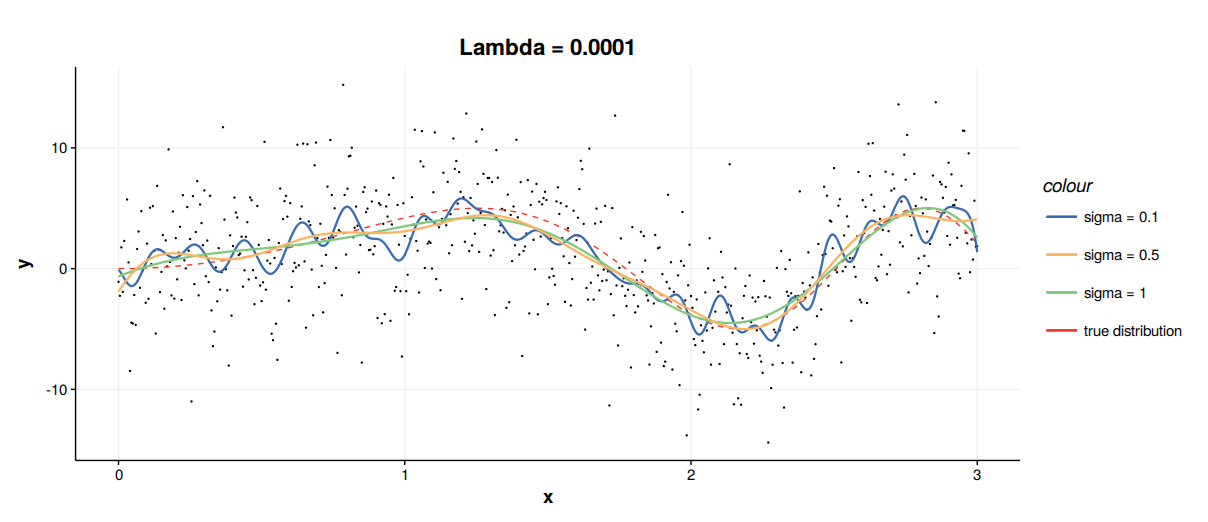
\includegraphics[width=6.7cm]{fig/0d0001.png}
	\end{subfigure}
	\begin{subfigure}{6.7cm}
		\centering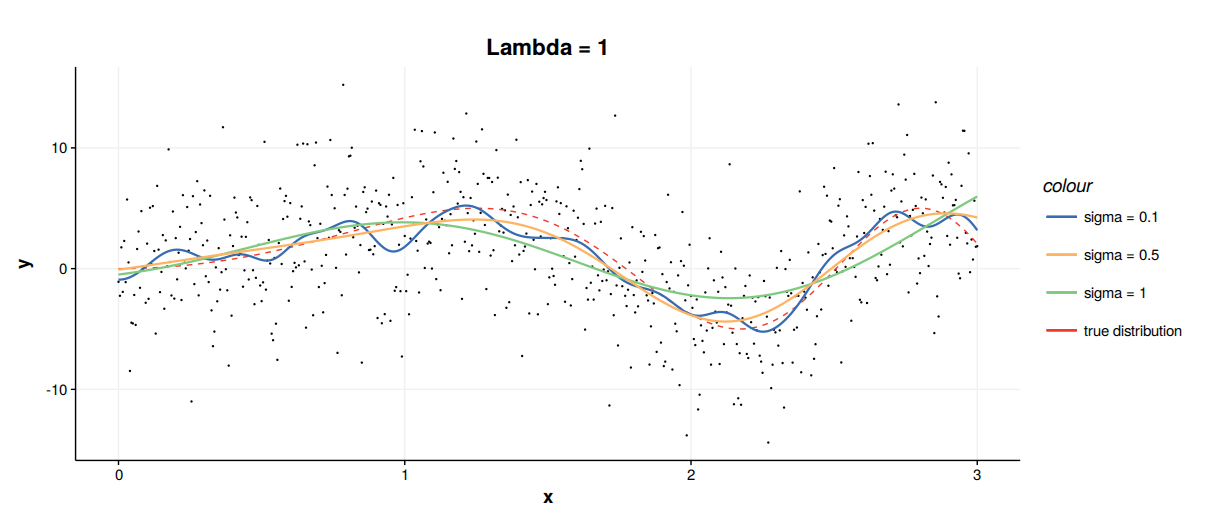
\includegraphics[width=6.7cm]{fig/1.png}
	\end{subfigure}
	\begin{subfigure}{6.7cm}
		\centering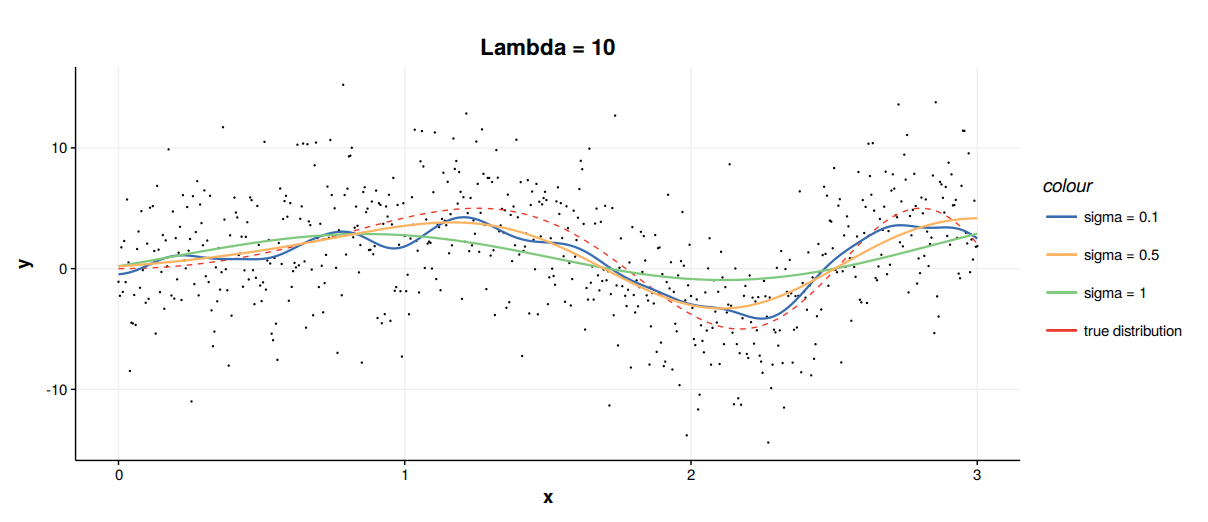
\includegraphics[width=6.7cm]{fig/10.png}
	\end{subfigure}
	\begin{subfigure}{6.7cm}
		\centering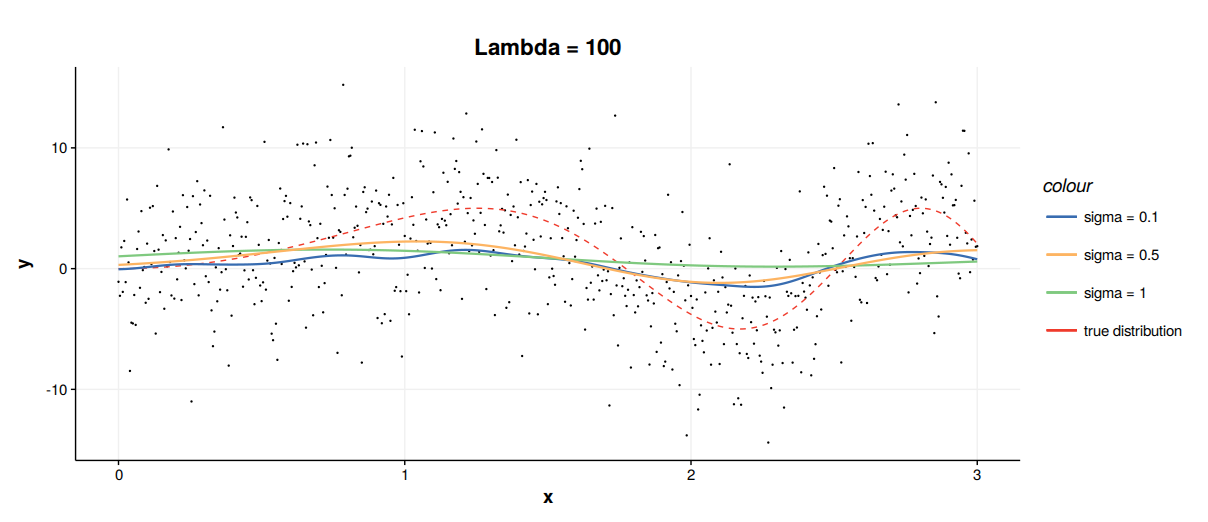
\includegraphics[width=6.7cm]{fig/100.png}
	\end{subfigure}
	\caption{Simulated data with respect to $y\sim f(x)+\varepsilon_i$, where $f(x)=5\sin(x^2)$ and $\varepsilon_i\sim\mathcal{N}(0,1)$. The parameter $\lambda$ controls how much we penalize lack of "smoothness" of $f$ - very low $\lambda$ might result in overfitting and very high values results in underfitting.}
\end{figure}

\sssection{Bounding the expected loss}
In the following, we will assume that all samples in $S_n$ are sampled i.i.d. from an unknown fixed distribution $p(X,Y)$. Let $\ell(y_1,y_2)$ denote a loss function. For a classification hypothesis $h \colon \mathcal{X}\to \R$, we define the \emph{expected risk}, $I(h)$, and the \emph{empirical risk}, $I_{S_n}(h)$, by
\begin{align*}
	I(h) &:= \int_{\mathcal{X}\times \R} \ell(h(x),y) \d p(x,y)\\
	I_{S_n}(h) &:= \frac{1}{n}\sum_{i = 1}^n \ell(h(x_i),y_i).
\end{align*}
We then define the \emph{generalization error}, $D_{S_n}(h)$, of $h$ to be $D_{S_n}(h):=I(h)-I_{S_n}(h)$.
\begin{definition}
	Let $H$ denote a class of hypotheses. A \emph{Generalization Bound} is any inequality such that for $\delta \in (0,1)$ it that
	\begin{align*}
		\mathbb{P}( |D_{S}(h)| \geq B(H,\delta,n,h) \text{ for some } h \in H) \leq \delta,
	\end{align*}	
	where $B(H,\delta,n,h)$ is a function of $h$ taking values in $(0,\infty)$ for fixed $H, \delta$ and sample size $n$.
\end{definition}
If one can choose $H=\H_k$ for some positive definite kernel $k$ and choose a function $B$ such that for fixed $\delta \in (0,1)$ and $n \geq 1$, the function $g \colon h \mapsto B(H,\delta,n,h)$ is only dependant on $\lv h\rv_{\H_k}$ and is a strictly increasing, then we can apply the representer theorem with $g(\lv h \rv_{\H_k})=B(H,\delta,n,h)$ so that with high probability, we bound the expected risk by reducing the empirical risk $I(h)$ when choosing $h$.

Applying Vapnik-Chervonenkis theory (see e.g. \cite{abu}), one can show that for the RKHS $\H_k$ of linear separators on $\R^n$ that the following holds:
\begin{theorem}
	Let $\H_k$ denote the RKHS of linear separators in $\R^n$ and let $\delta \in (0,1)$. Then
	\begin{align*}
		\mathbb{P}\left( \exists h=(w,b) \mid |D_{S}(h)|\geq \sqrt{\frac{8 \ln\left( 2( (2n)^{1+\lceil 1 \lv w \rv^2 \rceil }+1 \right)(1+\lceil \lv w \rv^2 \rceil)\lceil \lv w \rv^2 \rceil \delta^{-1}}{n}}\right) \leq \delta,
	\end{align*}
	where the size of $S=n$, where the loss functional $\ell$ is the $0-1$ loss and the target samples $y \in  \{\pm 1 \}$, and the notation that for $h=(w,b)$ we mean $h(x)=\mathrm{sgn}(\langle w,x \rangle+b)$.
\end{theorem}

For further reading we refer to \cite{genbd}, and for a concrete example in the choice of $g$, we refer to the theory of pattern recognition found in \cite{vapnik}.
\sssection{Support Vector Machine formulation}
A popular and empirically effective algorithm for classification is the Support Vector Machine (SVM). We now show why the representer theorem ensures that the SVM problems have a "nice" formulation. Let us first state the kernel SVM problem for some positive definite kernel $k$: Let $(x_1,y_1),\dots,(x_n,y_n)$ be given with $y_j \in \{ \pm 1 \}$ for $j = 1,2,\dots,n$. Then the SVM problem formulation without offset is:
\begin{align}
	\min_{f \in \H_k} \frac{1}{n} \sum_{i=1}^n \ell_{hinge}(y_i f(x_i)) + \lambda \lv f \rv_{\H_k}^2, \label{svmform1}
\end{align}
where $\ell_{hinge}(u) = \max(1-u,0)$ and $\lambda >0$. By \Cref{NPRT}, this is equivalent to
\begin{align*}
	\min_{\pmb \alpha \in \R^n}  \frac{1}{n} \sum_{i=1}^n \ell_{hinge}(y_i \pi_i(\textbf{K} \pmb \alpha))+ \lambda \pmb \alpha^T \textbf{K} \pmb \alpha,
\end{align*}
where $\pi_i$ denotes the $i'th$ coordinate projection map. This is not a smooth problem by the involvement of $\ell_{hinge}$. To deal with this, using Lagrangian theory and forming the Primal formulation of the problem and then its corresponding dual formulation, one can arrive that the equivalent formulation of \Cref{svmform1} given by:
\begin{align*}
&&	&\max_{\pmb \alpha \in \R^n} &  &2 \pmb \alpha^T \pmb y - \pmb \alpha^T \pmb K \pmb \alpha\\
&&	&\text{such that } & &0 \leq y_i \alpha_i \leq (2 \lambda n)^{-1}, \ i = 1,2,\dots,n.
\end{align*}
This formulation is a Quadratic Programming Problem, which can be solved numerically using different algorithms. For the specific proofs regarding the arrival at the Dual formulation, we refer to e.g. \cite{smola}.
\printbibliography

\end{document}


